\chapter{第二部分}
\section{问题概述}
%
%%对问题的直观描述
%
%
%对项目已有代码的阅读和理解
%
%
%解决问题的思路和想法
%
该部分包含第3、4、5小题。

该部分中要求我们通过完成pacmanSuccessorAxiomSingle和pacphysicsAxioms来对吃豆人游戏规则进行建模。在此基础之上完成checkLocationSatisfiability,
其功能是给定上一时刻的吃豆人位置,判断下一时刻吃豆人是否有可能(不)达到指定位置,如果有可能,返回一个满足的模型,否则返回False。然后,我们需要利用逻辑来帮助吃豆人规划从起始位置到目标位置的路线。最后,需要
利用逻辑来帮助吃豆人规划收集所有食物的方案。
\section{算法设计}
%
%用自己的语言描述解决问题所使用的算法的原理及功能,设计思路和算法流程图
%
参考SLAMSuccessorAxiomSingle,pacmanSuccessorAxiomSingle用于描述吃豆人如何在时刻$t$时到达$(x,y)$处。由于这里不允许吃豆人停止,该事件发生当且仅当
吃豆人上一时刻在相邻位置,并且在上一时刻朝着该位置移动。

按照题目要求,pacphysicsAxioms中需要包含以下内容:
\begin{enumerate}
    \item 对于所有的坐标,“有墙”蕴含着“吃豆人不在这里”
    \item 在每一时刻吃豆人恰好在一个位置(这可以通过exactlyOne函数实现)
    \item 在每一时刻吃豆人恰好执行一个动作(这可以通过exactlyOne函数实现)
    \item sensorModel返回的语句
    \item successorAxioms返回的语句
\end{enumerate}

按照题目要求,在checkLocationSatisfiablity中,首先向知识库KB中添加以下内容:
\begin{enumerate}
    \item pacphysics\_axioms返回值
    \item 吃豆人初始位置
    \item 吃豆人执行了action0
    \item 吃豆人执行了action1
\end{enumerate}
这里action0和action1分别是在时刻0和时刻1执行。这里的action1的用途只是为了确保由SAT返回的模型和autograder中设定的一致。由于需要返回
具体的模型,所以最后需要调用findModel,将KB以及询问的内容,即吃豆人在时刻1(不)位于指定位置,传入。

positionLogicPlan算法的伪代码在下一页中给出。核心思想是:每一时刻,添加对于吃豆人位置的约束,然后判断吃豆人在当前时刻达到目标位置,如果能,
则返回对应的行动,否则,添加该时刻中对于吃豆人动作的约束,以及转移公理,从而完成了从这一时刻到下一时刻的过渡。

\begin{algorithm}
    \SetKw{in}{in}
    \SetKw{print}{print}
    \SetKw{range}{range}
    KB = []\;
    KB.append(pacmanInitialLocation)\;
    \For{t \in \range(50)}
    {
        \print(t)\tcp*[h]{因为运行时间较长,用于获取当前进度}\;
        KB.append(pacmanInExactlyOneLocationSentence(t))\tcp*[h]{吃豆人恰好在一个位置}\;
        result = findModel(KB+pacmanInGoalPositionSentence(t))\tcp*[h]{是否存在模型,其中吃豆人到达目标位置}\;
        \If(\tcp*[h]{存在解,则从中提取行动序列}){result}{\Return{extractActionSequence(result)}}
        KB.append(pacmanTakeExactlyOneActionSentenc(t))\tcp*[h]{吃豆人恰好执行一个动作}\;
        \ForAll{coordinate \in non\_wall\_coords}
        {
        KB.append(pacmanSuccessorAxiomsSingle(coordinate,t+1))\tcp*[h]{转移公理}\;
        }
    }
    \caption{positionLogiPlan}
\end{algorithm}

% \begin{algorithm}
%     \SetKw{in}{in}
%     \SetKw{print}{print}
%     \SetKw{range}{range}
%     KB = []\;
%     KB.append(pacmanInitialLocation)\;
%     \ForAll{food \in foods}
%     {
%         KB.append(food.positionSentence(0))\;
%     }
%     \For{t \in \range(50)}
%     {
%         \print(t)\tcp*[h]{因为运行时间较长,用于获取当前进度}\;
%         KB.append(pacmanInExactlyOneLocationSentence(t))\tcp*[h]{吃豆人恰好在一个位置}\;
%         goalSentence = []\;
%         \ForAll{food \in foods}
%         {
%             goalSentence.append($\lnot$food.positionSentence(t))\;
%         }
%         result = findModel(KB+goalSentence)\tcp*[h]{是否存在模型,其中不存在任何食物}\;
%         \If(\tcp*[h]{存在解,则从中提取行动序列}){result}{\Return{extractActionSequence(result)}}
%         KB.append(pacmanTakeExactlyOneActionSentenc())\tcp*[h]{吃豆人恰好执行一个动作}\;
%         \ForAll{coordinate \in non\_wall\_coords}
%         {
%         KB.append(pacmanSuccessorAxiomsSingle(coordinate,t+1))\tcp*[h]{转移公理}\;
%         KB.append(foodSuccessorAxiomsSingle(coordinate,t+1))\tcp*[h]{转移公理}\;
%         }
%     }
%     \caption{foodLogicPlan}
% \end{algorithm}

foodLogicPlan算法的整体逻辑以及伪代码和positionLogicPlan的类似。区别在于,知识库KB初始化时,需要添加食物的初始信息。同时,
判断给定时刻是否存在解的条件时该时刻的吃豆人收集掉了所有食物,即此时地图中没有任何食物存在。并且,两个时刻之间的状态不仅仅
由pacmanSuccessorAxiom进行约束,还需要利用foodSuccessorAxiom对食物的状态进行约束,即:给定一个位置,如果在上一时刻没有食物,在这一时刻也没有食物;
如果在上一时刻有食物,那么如果这一时刻吃豆人在该位置上,这一时刻便没有食物了,否则仍然有食物。

\section{算法实现}
%
%在算法原理的基础上,结合代码,讲述算法的实现细节、和兴函数、模块输入输出,数据结构定义等内容
%

在pacphysicsAxioms函数中,只有当t不为0时,才有可能向KB中添加这一时刻的转移公理,这是因为对于初始时刻而言,并没有上一时刻,自然不受转移公理的约束。

在checkLocationSatisfiability,positionLogicPlan和foodLogicPlan函数中,查询某一结论是否存在模型满足它时,需要将KB和结论合取在一起,然后
传入findModel函数中。这里需要注意的是,结论并不属于KB的一部分,所以不能将其添加进KB中,只能采用临时变量,即运算符+返回的结果,作为参数传入
findModel函数中。

在positionLogicPlan和foodLogicPlan函数中,并没有调用先前实现的pacphysicsAxioms函数,而是将其拆分开来。主要原因是因为pacphysicsAxiom函数
相当于把时间的每一刻视为一个整体,但是在这两个函数中,我们在每一刻中执行的操作是有先后顺序的。由于转移公理描述的是给定时刻受上一时刻的约束,
所以在循环体内,传入转移公理的时刻都是$t+1$,而非$t$,因为下一轮循环便进入了$t+1$时刻。

以下为算法的具体实现,其中略去了已给的部分代码。
\begin{lstlisting}[emph={[3]x,y,time,sensorModel,successorAxioms,action0,action1,problem},emphstyle={[3]\color{vscode_parametercolor}},emph={[4]Expr,SearchProblem,Callable,Node,Actions,Reached,Any,List,Tuple},emphstyle={[4]\color{vscode_classcolor}}]
def pacmanSuccessorAxiomSingle(x: int, y: int, time: int, walls_grid: List[List[bool]] = None) -> Expr:
    # 略去已给代码
    return PropSymbolExpr(pacman_str, x, y, time=time) % disjoin([possible_cause for possible_cause in possible_causes])

def pacphysicsAxioms(t: int, all_coords: List[Tuple], non_outer_wall_coords: List[Tuple], walls_grid: List[List] = None, sensorModel: Callable = None, successorAxioms: Callable = None) -> Expr:
    pacphysics_sentences = []

    notInWall = [PropSymbolExpr(wall_str, x, y) >> ~PropSymbolExpr(pacman_str, x, y, time=t) for x, y in all_coords]
    inExactOne = exactlyOne([PropSymbolExpr(pacman_str, x, y, time=t) for x, y in non_outer_wall_coords])
    doExactOne = exactlyOne([PropSymbolExpr(direction, time=t) for direction in DIRECTIONS])
    pacphysics_sentences += notInWall
    pacphysics_sentences.append(inExactOne)
    pacphysics_sentences.append(doExactOne)
    if sensorModel:
        pacphysics_sentences.append(sensorModel(t, non_outer_wall_coords))
    if t and successorAxioms: # 初始时刻并不受上一时刻的约束
        pacphysics_sentences.append(successorAxioms(t, walls_grid, non_outer_wall_coords))

    return conjoin(pacphysics_sentences)

def checkLocationSatisfiability(x1_y1: Tuple[int, int], x0_y0: Tuple[int, int], action0, action1, problem):
    # 略去已给代码

    map_sent = [PropSymbolExpr(wall_str, x, y) for x, y in walls_list]
    KB.append(conjoin(map_sent))

    KB.append(pacphysicsAxioms(0, all_coords, non_outer_wall_coords, walls_grid, None, allLegalSuccessorAxioms))
    KB.append(pacphysicsAxioms(1, all_coords, non_outer_wall_coords, walls_grid, None, allLegalSuccessorAxioms))
    KB.append(PropSymbolExpr(pacman_str, x0, y0, time=0))
    KB.append(PropSymbolExpr(action0, time=0))
    KB.append(PropSymbolExpr(action1, time=1))

    inx1_y1 = findModel(conjoin(KB + [PropSymbolExpr(pacman_str, x1, y1, time=1)]))
    notInx1_y1 = findModel(conjoin(KB + [~PropSymbolExpr(pacman_str, x1, y1, time=1)]))
    return inx1_y1, notInx1_y1

def positionLogicPlan(problem) -> List:
    # 略去已给代码
    KB = []
    KB.append(PropSymbolExpr(pacman_str, x0, y0, time=0))
    for t in range(0, 50):
        print(t)
        KB.append(exactlyOne([PropSymbolExpr(pacman_str, x, y, time=t) for x, y in non_wall_coords]))
        result = findModel(conjoin(KB + [PropSymbolExpr(pacman_str, xg, yg, time=t)]))
        if result:
            return extractActionSequence(result, actions)
        KB.append(exactlyOne([PropSymbolExpr(action, time=t) for action in actions]))
        KB += [pacmanSuccessorAxiomSingle(x, y, t + 1, walls_grid) for x, y in non_wall_coords]

def foodSuccessorAxiomSingle(x: int, y: int, time: int, walls_grid: List[List[bool]] = None) -> Expr:
    now, last = time, time - 1
    return conjoin([
        ~PropSymbolExpr(food_str, x, y, time=last) >> ~PropSymbolExpr(food_str, x, y, time=now),  # 没有食物的位置不会生成食物
        conjoin(
            [PropSymbolExpr(food_str, x, y, time=last), PropSymbolExpr(pacman_str, x, y, time=now)]) >> ~PropSymbolExpr(
            food_str, x, y, time=now),
        # 移动到有食物的位置后,食物便消失了
        conjoin(
            [PropSymbolExpr(food_str, x, y, time=last), ~PropSymbolExpr(pacman_str, x, y, time=now)]) >> PropSymbolExpr(
            food_str, x, y, time=now),
        # 如果没有吃豆人移动到有食物的位置,那么该位置仍然有食物
    ])

def foodLogicPlan(problem) -> List:
    # 略去已给代码
    KB = []
    KB.append(PropSymbolExpr(pacman_str, x0, y0, time=0))
    KB += [PropSymbolExpr(food_str, x, y, time=0) for x, y in food]
    for t in range(0, 50):
        print(t)
        KB.append(exactlyOne([PropSymbolExpr(pacman_str, x, y, time=t) for x, y in non_wall_coords]))
        result = findModel(conjoin(KB + [~PropSymbolExpr(food_str, x, y, time=t) for x, y in food]))
        if result:
            return extractActionSequence(result, actions)
        KB.append(exactlyOne([PropSymbolExpr(action, time=t) for action in actions]))
        KB += [pacmanSuccessorAxiomSingle(x, y, t + 1, walls) for x, y in non_wall_coords]
        KB += [foodSuccessorAxiomSingle(x, y, t + 1, walls) for x, y in food]
\end{lstlisting}
\section{实验结果}
\subsection{Question3}
成功通过Question3的全部测试,实验结果截图见图\ref{q3}。
这里所使用的到的测试用例较为基础,检查了上述函数是否能够返回正确的结果。
\begin{figure}[htbp]
    \centering
    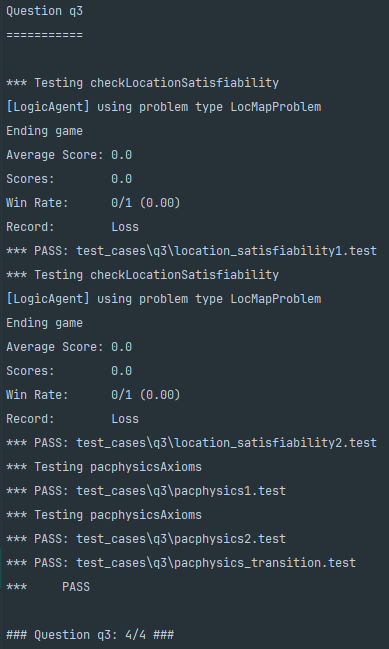
\includegraphics[scale = 0.7]{pic/q3.png}
    \caption{Question3实验结果}\label{q3}
\end{figure}
\subsection{Question4}
成功通过Question4的全部测试,实验结果截图见图\ref{q412},\ref{q43}。
所用到的测试样例便是将吃豆人放在迷宫场景中进行实战,三个测试样例中的迷宫大小递增。
\begin{figure}[!htbp]
    \centering
    \begin{minipage}[t]{0.4\textwidth}
    \centering
    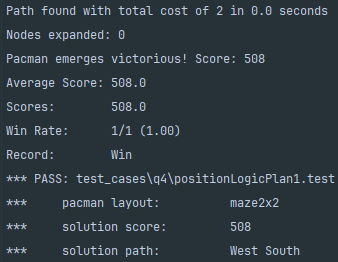
\includegraphics[width=\textwidth]{pic/q41.png}
    \end{minipage}
    \begin{minipage}[t]{0.55\textwidth}
    \centering
    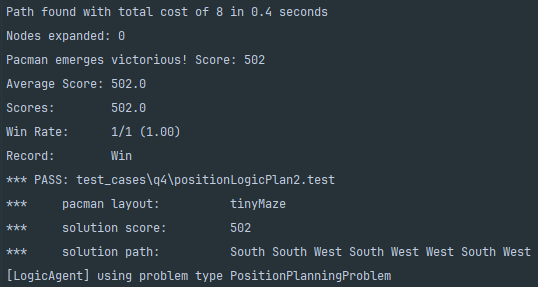
\includegraphics[width=\textwidth]{pic/q42.png}
    \end{minipage}
    \caption{Question4实验结果}\label{q412}
\end{figure}
\begin{figure}[htbp]
    \centering
    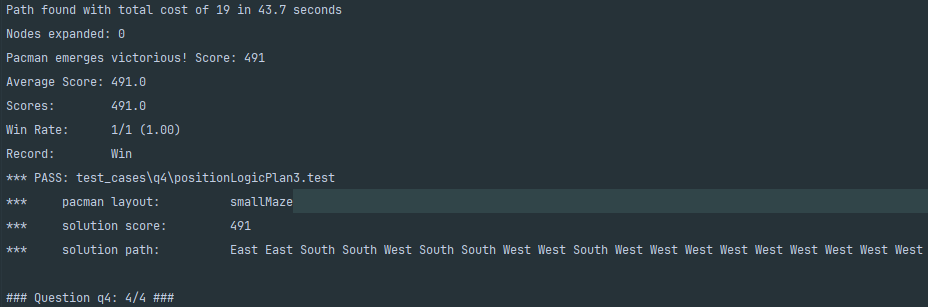
\includegraphics[width = \textwidth]{pic/q43.png}
    \caption{Question4实验结果}\label{q43}
\end{figure}
\subsection{Question5}
成功通过Question5的全部测试,实验结果截图见图\ref{q51},\ref{q52}。
所用到的测试样例便是将吃豆人放在迷宫场景中进行实战,两个测试样例中的迷宫大小递增,食物数量也递增。
\begin{figure}[htbp]
    \centering
    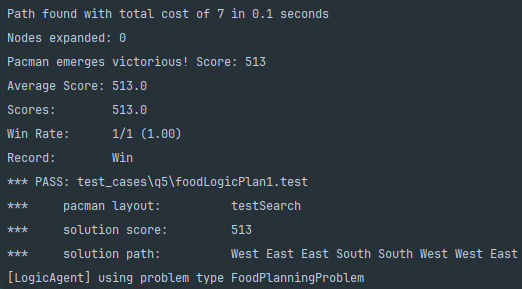
\includegraphics[scale = 0.8]{pic/q51.png}
    \caption{Question5实验结果}\label{q51}
\end{figure}
\begin{figure}[htbp]
    \centering
    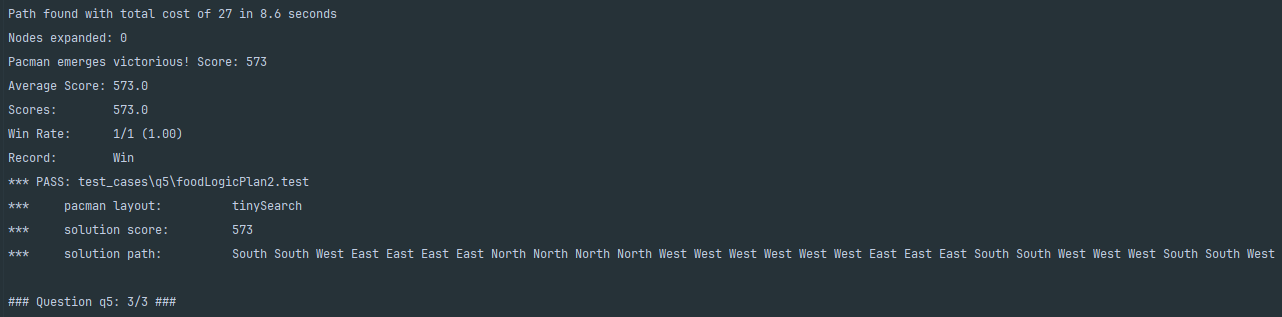
\includegraphics[width = \textwidth]{pic/q52.png}
    \caption{Question5实验结果}\label{q52}
\end{figure}
%
%对试验结果进行详细展示,对每个问题展示测试截图,对于测试用例进行描述说明,对于为通过测试的用例结合自己的算法进行分析,可以结合调试过程进行分析
%
%实验中遇到的问题及解决方案,收获和思考:对算法的理解、优缺点的评价、算法的适用场景
%
